\begin{figure}[t]
\centering
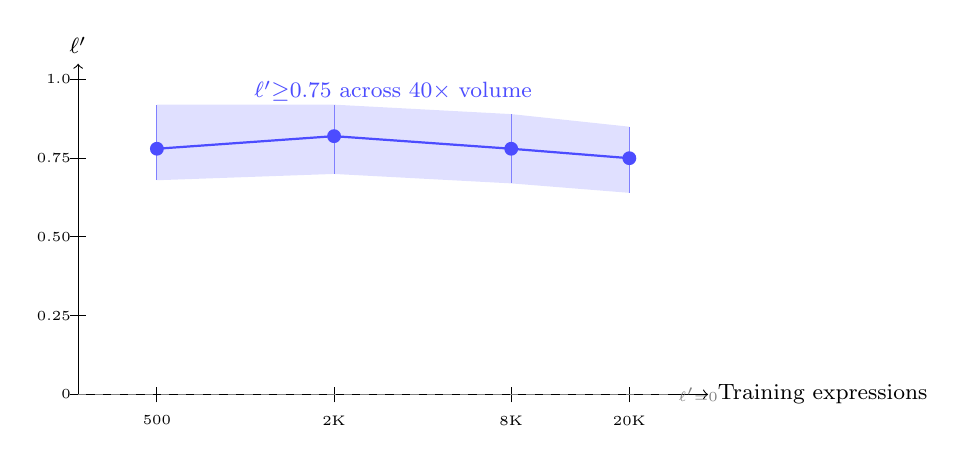
\begin{tikzpicture}[font=\small]

% Axes
\draw[->] (0, 0) -- (0, 4.2) node[above, font=\footnotesize] {$\ell'$};
\draw[->] (0, 0) -- (8.0, 0) node[right, font=\footnotesize] {Training expressions};

% Y ticks (ell' from 0 to 1.0, scale: 4cm = 1.0)
\foreach \yv/\ylbl in {0/0, 1/0.25, 2/0.50, 3/0.75, 4/1.0} {
  \draw (-0.1, \yv) -- (0.1, \yv) node[left, font=\tiny, xshift=-2pt] {\ylbl};
}

% X positions (log scale: 500, 2K, 8K, 20K)
% log10(500)=2.70, log10(2000)=3.30, log10(8000)=3.90, log10(20000)=4.30
% Map [2.7, 4.3] to [1.0, 7.0]: x = (log10(N) - 2.7) * (6.0/1.6) + 1.0
\def\xA{1.0}    % 500
\def\xB{3.25}   % 2000
\def\xC{5.50}   % 8000
\def\xD{7.0}    % 20000

% X tick labels
\foreach \xp/\xlbl in {\xA/500, \xB/2K, \xC/8K, \xD/20K} {
  \draw (\xp, -0.1) -- (\xp, 0.1);
  \node[below, font=\tiny] at (\xp, -0.15) {\xlbl};
}

% Actual ell' values from experiments:
% 500: 0.78 [0.68, 0.92]
% 2000: 0.82 [0.70, 0.92]
% 8000: 0.78 [0.67, 0.89]
% 20000: 0.75 [0.64, 0.85]
% y positions (ell' * 4):
\def\yA{3.12}  % 0.78
\def\yB{3.28}  % 0.82
\def\yC{3.12}  % 0.78
\def\yD{3.00}  % 0.75

% CI bands
% 500: [0.68, 0.92] -> [2.72, 3.68]
% 2000: [0.70, 0.92] -> [2.80, 3.68]
% 8000: [0.67, 0.89] -> [2.68, 3.56]
% 20000: [0.64, 0.85] -> [2.56, 3.40]
\fill[blue!12]
  (\xA, 3.68) -- (\xB, 3.68) -- (\xC, 3.56) -- (\xD, 3.40)
  -- (\xD, 2.56) -- (\xC, 2.68) -- (\xB, 2.80) -- (\xA, 2.72) -- cycle;

% Main curve
\draw[thick, blue!70] (\xA, \yA) -- (\xB, \yB) -- (\xC, \yC) -- (\xD, \yD);

% Data points with error bars
\foreach \xp/\yp/\ylo/\yhi in {\xA/3.12/2.72/3.68, \xB/3.28/2.80/3.68, \xC/3.12/2.68/3.56, \xD/3.00/2.56/3.40} {
  \draw[blue!50] (\xp, \ylo) -- (\xp, \yhi);
  \fill[blue!70] (\xp, \yp) circle (2.5pt);
}

% Reference line (no-leakage baseline)
\draw[dashed, gray] (0, 0) -- (7.5, 0) node[right, font=\tiny, gray] {$\ell'{=}0$};

% Annotation
\node[font=\footnotesize, align=center, blue!70] at (4.0, 3.85) {$\ell'{\geq}0.75$ across $40\times$ volume};

\end{tikzpicture}
\caption{Augmentation-volume robustness (E3b protocol, Tree-LSTM, $n{=}10$/$5$/$5$/$25$ seeds at 500/2K/8K/20K respectively, bootstrap 95\% CIs). $\ell'$ remains high (${\geq}0.75$) at every volume tested. The 20K point derives from tag \texttt{r34}; 500--8K points from \texttt{r39b/d/f}. Between-run-family differences (${\sim}0.10$) exceed any volume effect, so we report levels rather than a fitted trend. More gradient exposure to paraphrases of the same equations does not teach variable-identity invariance.}
\label{fig:scale_curve}
\end{figure}
